\documentclass[11pt,preprint, authoryear]{elsarticle}

\usepackage{lmodern}
%%%% My spacing
\usepackage{setspace}
\setstretch{1.2}
\DeclareMathSizes{12}{14}{10}{10}

% Wrap around which gives all figures included the [H] command, or places it "here". This can be tedious to code in Rmarkdown.
\usepackage{float}
\let\origfigure\figure
\let\endorigfigure\endfigure
\renewenvironment{figure}[1][2] {
    \expandafter\origfigure\expandafter[H]
} {
    \endorigfigure
}

\let\origtable\table
\let\endorigtable\endtable
\renewenvironment{table}[1][2] {
    \expandafter\origtable\expandafter[H]
} {
    \endorigtable
}


\usepackage{ifxetex,ifluatex}
\usepackage{fixltx2e} % provides \textsubscript
\ifnum 0\ifxetex 1\fi\ifluatex 1\fi=0 % if pdftex
  \usepackage[T1]{fontenc}
  \usepackage[utf8]{inputenc}
\else % if luatex or xelatex
  \ifxetex
    \usepackage{mathspec}
    \usepackage{xltxtra,xunicode}
  \else
    \usepackage{fontspec}
  \fi
  \defaultfontfeatures{Mapping=tex-text,Scale=MatchLowercase}
  \newcommand{\euro}{€}
\fi

\usepackage{amssymb, amsmath, amsthm, amsfonts}

\def\bibsection{\section*{References}} %%% Make "References" appear before bibliography


\usepackage[round]{natbib}

\usepackage{longtable}
\usepackage[margin=2.3cm,bottom=2cm,top=2.5cm, includefoot]{geometry}
\usepackage{fancyhdr}
\usepackage[bottom, hang, flushmargin]{footmisc}
\usepackage{graphicx}
\numberwithin{equation}{section}
\numberwithin{figure}{section}
\numberwithin{table}{section}
\setlength{\parindent}{0cm}
\setlength{\parskip}{1.3ex plus 0.5ex minus 0.3ex}
\usepackage{textcomp}
\renewcommand{\headrulewidth}{0pt}

\usepackage{array}
\newcolumntype{x}[1]{>{\centering\arraybackslash\hspace{0pt}}p{#1}}

%%%%  Remove the "preprint submitted to" part. Don't worry about this either, it just looks better without it:
\makeatletter
\def\ps@pprintTitle{%
  \let\@oddhead\@empty
  \let\@evenhead\@empty
  \let\@oddfoot\@empty
  \let\@evenfoot\@oddfoot
}
\makeatother

 \def\tightlist{} % This allows for subbullets!

\usepackage{hyperref}
\hypersetup{breaklinks=true,
            bookmarks=true,
            colorlinks=true,
            citecolor=blue,
            urlcolor=blue,
            linkcolor=blue,
            pdfborder={0 0 0}}


% The following packages allow huxtable to work:
\usepackage{siunitx}
\usepackage{multirow}
\usepackage{hhline}
\usepackage{calc}
\usepackage{tabularx}
\usepackage{booktabs}
\usepackage{caption}


\newenvironment{columns}[1][]{}{}

\newenvironment{column}[1]{\begin{minipage}{#1}\ignorespaces}{%
\end{minipage}
\ifhmode\unskip\fi
\aftergroup\useignorespacesandallpars}

\def\useignorespacesandallpars#1\ignorespaces\fi{%
#1\fi\ignorespacesandallpars}

\makeatletter
\def\ignorespacesandallpars{%
  \@ifnextchar\par
    {\expandafter\ignorespacesandallpars\@gobble}%
    {}%
}
\makeatother

\newlength{\cslhangindent}
\setlength{\cslhangindent}{1.5em}
\newenvironment{CSLReferences}%
  {\setlength{\parindent}{0pt}%
  \everypar{\setlength{\hangindent}{\cslhangindent}}\ignorespaces}%
  {\par}


\urlstyle{same}  % don't use monospace font for urls
\setlength{\parindent}{0pt}
\setlength{\parskip}{6pt plus 2pt minus 1pt}
\setlength{\emergencystretch}{3em}  % prevent overfull lines
\setcounter{secnumdepth}{5}

%%% Use protect on footnotes to avoid problems with footnotes in titles
\let\rmarkdownfootnote\footnote%
\def\footnote{\protect\rmarkdownfootnote}
\IfFileExists{upquote.sty}{\usepackage{upquote}}{}

%%% Include extra packages specified by user

%%% Hard setting column skips for reports - this ensures greater consistency and control over the length settings in the document.
%% page layout
%% paragraphs
\setlength{\baselineskip}{12pt plus 0pt minus 0pt}
\setlength{\parskip}{12pt plus 0pt minus 0pt}
\setlength{\parindent}{0pt plus 0pt minus 0pt}
%% floats
\setlength{\floatsep}{12pt plus 0 pt minus 0pt}
\setlength{\textfloatsep}{20pt plus 0pt minus 0pt}
\setlength{\intextsep}{14pt plus 0pt minus 0pt}
\setlength{\dbltextfloatsep}{20pt plus 0pt minus 0pt}
\setlength{\dblfloatsep}{14pt plus 0pt minus 0pt}
%% maths
\setlength{\abovedisplayskip}{12pt plus 0pt minus 0pt}
\setlength{\belowdisplayskip}{12pt plus 0pt minus 0pt}
%% lists
\setlength{\topsep}{10pt plus 0pt minus 0pt}
\setlength{\partopsep}{3pt plus 0pt minus 0pt}
\setlength{\itemsep}{5pt plus 0pt minus 0pt}
\setlength{\labelsep}{8mm plus 0mm minus 0mm}
\setlength{\parsep}{\the\parskip}
\setlength{\listparindent}{\the\parindent}
%% verbatim
\setlength{\fboxsep}{5pt plus 0pt minus 0pt}



\begin{document}



\begin{frontmatter}  %

\title{The Church as a Lending Institution in the Cape Colony 1670 -
1710}

% Set to FALSE if wanting to remove title (for submission)




\author[Add1]{Harriet Catherine Laing}
\ead{21617023@sun.ac.za}





\address[Add1]{Stellenbosch University, Stellenbosch, South Africa}



\vspace{1cm}





\vspace{0.5cm}

\end{frontmatter}



%________________________
% Header and Footers
%%%%%%%%%%%%%%%%%%%%%%%%%%%%%%%%%
\pagestyle{fancy}
\chead{}
\rhead{}
\lfoot{}
\rfoot{\footnotesize Page \thepage}
\lhead{}
%\rfoot{\footnotesize Page \thepage } % "e.g. Page 2"
\cfoot{}

%\setlength\headheight{30pt}
%%%%%%%%%%%%%%%%%%%%%%%%%%%%%%%%%
%________________________

\headsep 35pt % So that header does not go over title




\hypertarget{introduction}{%
\section{\texorpdfstring{Introduction
\label{Introduction}}{Introduction }}\label{introduction}}

Upon the arrival of the first Dutch settlers in the Cape, came the
establishment of religious institutions that impacted the economy. The
Cape Colony was first established in 1652 by Jan van Riebeeck to serve
as a refreshment station for Vereenigde Oostindische Compagnie (VOC)
ships. In order to fulfill the objective of the VOC to provide fresh
produce to passing ships, the VOC provided land and loans new settlers.
The church also provided loans in the early years of the Cape Colony.
The role of the church as a lending institution is not well understood.
However, this paper begins to determine the influence of church loans
for individual loan recipients in the Cape Colony at a time when the
first settlers were beginning to establish farming ventures and their
new lives in the Cape.

Society in the Cape Colony was heterogenous in terms of the origins of
the settlers, as well as their slaves, and their wealth. This paper
sought to determine whether there is an effect of the type of individual
loan recipients on the loan amount that the church granted. Section 2
provides brief background on the establishment of the Cape Colony, the
different groups within the society during this time period, and
outlines the role of the church in the literature. Section 3 presents
the data set used in this paper's analysis and section 4 explains the
methodology applied to answer the main research question. Section 5
provides the limitations of this paper and, lastly, section 6 concludes.

\hypertarget{background}{%
\section{\texorpdfstring{Background
\label{Literature}}{Background }}\label{background}}

The VOC was a company that was chartered by the Dutch Republic's State
General to act on behalf of its colonised territories overseas (Fourie
\emph{et al}. 2012:51). The Cape was colonised to address the high
incidence of scurvy that the VOC sailors were prone to falling sick to,
while on long ship voyages between Holland and the East Indies (Fourie
\emph{et al}. 2012:55). The first settler population that inhabited the
Cape consisted of approximately two hundred individuals. A large
proportion of these first settlers were male, whereas women and children
constituted only five percent of the settlers' population recorded in
1658 (Horner \& Wilson, 2008:8). In the same year, slaves constituted 52
percent of the population; approximately half of which were owned by the
VOC and the other half owned by freemen (Horner \& Wilson, 2008:8). By
1701, the population had grown to approximately 4 500 (at least based on
those involved in the Cape economy) as more European immigrants and
slaves arrived in the Cape (Fourie \& Luiten van Zanden, 2012).

Society in the Cape Colony consisted of four main groups, namely (i) the
settler population, (ii) the VOC officials and employees, (iii) the
Khoesan (the original inhabitants of the Cape) and (iv) slaves. The
settler population consisted primarily of Dutch and German people from a
variety of socio-economic backgrounds; some were affluent or ``middle
class'' with debt burdens, and others poor and without land (Guelke,
1988:458). There was a further group included in the settler population
that originated from France. These immigrants were known as Huguenots
and had fled because of the increased persecution of Protestants in
their origin country (Horner \& Wilson, 2008:14). In the 1680s, many
Huguenots were offered a free passage to the Cape and advances for
equipment that they would use upon arrival by the VOC. These inducements
were provided upon the condition that the Huguenots pledged an oath of
allegiance to the VOC and remain there for at least five years (Horner
\& Wilson, 2008:14). The Huguenots were regarded by the VOC as a
potential asset to the Cape Colony, which is why they offered
inducements to this group to emigrate to the Cape (Wirgman, 1895:36).

Slaves first arrived at the Cape in a small group in the year following
1652. In 1654, the first slaving expedition by the VOC from the Cape
obtained more slaves to bring back from Madagascar (Horner \& Wilson,
2008:5). Slaves were rarely allowed to become manumitted. However,
slaves could have their freedom purchased if a free man wished to marry
them. For example, a notable marriage through which one female slave was
manumitted was between a woman called Eva and a free man called Pieter
van Meerhof (Horner \& Wilson, 2008:9). It is likely that she is the
recorded ``Eva de Hottentotin'' in the data set, as it is recorded that
van Meerhof predeceased Eva before 1674. Therefore, the dates align and
women tended to receive loans from the church on behalf of their late
husbands.

It is well-documented that the VOC provided land and loans to settlers
that arrived in the Cape. For example, in 1657, the directors of the VOC
mandated that nine married, settler couples from Dutch and German origin
be given farmlands in an attempt to provide a steady supply of meat,
grain and wine, following unsuccessful efforts in this regard by VOC
slaves (Horner \& Wilson, 2008:7). Generally, these first farmers in the
Cape Colony were previously servants for the VOC that were manumitted.
As they were previously servants, they had little resources or capital
to use in their new farming ventures. Accordingly, the VOC provided some
tools and cattle, however, any investments that were required in excess
of these items had to come from the farmers themselves (Fourie \& Von
Fintel, 2009:8).

It is less clear how the church served as a lending institution in the
early Cape Colony. It has been recorded that the church played a role in
giving money to farmers in need (Fourie \& Von Fintel, 2009:8). In 1665,
the first formal religious institution for the Dutch Reformed Consistory
was established at the Cape (Wirgman, 1895:23) and the Dutch Reformed
Church in Cape Town was completed in 1703 (Wirgman, 1895:31). The church
addressed matters that were notnot only religious but also related to
the control of government. The church was documented to assist needy
individuals financially, as the deacons of the Dutch Reformed church
helped destitute individuals and orphans (Wirgman, 1895:29). It is
uncertain how much wealth the church had throughout the period of
interest, but in 1679 it was recorded that the church had a capital fund
of 1535 British pounds available for charitable needs (Wirgman,
1895:29). However, the literature on the role of church as an economic
institution to provide loans for farmers and those in need of capital
for commercial ventures in the Cape is scarce.

\hypertarget{data}{%
\section{\texorpdfstring{Data \label{Data}}{Data }}\label{data}}

The data set used for this research were the 17 loan books of the church
in the Cape Colony spanning from 1670 to 1710, with some years missing.
Each loan book detailed the name of the loan recipient, the amount of
the loan (in gulden which was the currency used during this time
period), any interest accrued and a brief description thereof. This data
set includes a lot of persistent entries, as there are many recurring
loan recipients and loans amounts. In other words, it appears that the
same people in the Cape Colony receive loans from the church year after
year. However, what is less clear is whether these recurring loan
recipients are receiving a similar amount from the church each year, or
whether in some instances the initial amount that is loaned is simply
repaid the following year, or is simply accruing interest.

\begin{center}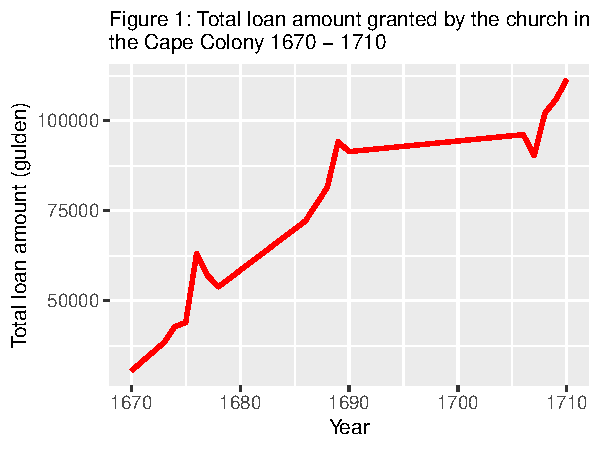
\includegraphics{HistoryEssay_files/figure-latex/unnamed-chunk-1-1} \end{center}

As can be seen in Figure 1, there was a general upward trend in the
total amount of loans provided by the church from 1670 until 1710. The
year 1687 was omitted from this graph as it was an unusually short loan
book, compared to the rest of the years in the data set, and distorted
the average change over time. Similarly, the year 1687 was dropped from
the number of loan recipients in Figure 2. From Figure 1, it is
evidenced that the church provided more loans over time. However, as
discussed in section 2, the population of the Cape Colony increased over
this time period, and there may have been inflationary pressures.
Therefore, this graph is insufficient to implicate that the influence of
the loans granted by the church increased over time.

Nevertheless, it is illustrated that the church increased its lending
capacity and had the ability to provide more capital to those living in
the Cape Colony in 1710 compared to 1670, an increase in excess of 70
000 gulden. As calculated by Fourie et al.~(2012) the VOC generated
approximately 50 000 gulden in the years of 1700 and 1705 from their
trading and commercial activities. For four years from 1670, the church
loaned 992 gulden to the VOC each year and then in 1706, the church
loaned the VOC 4000 gulden. The amounts recorded in the church loan
books may not have contributed much to the VOC itself, relative to its
revenue. However, it appears that the church and the VOC had close links
and that the church had significant wealth to lend.

\begin{center}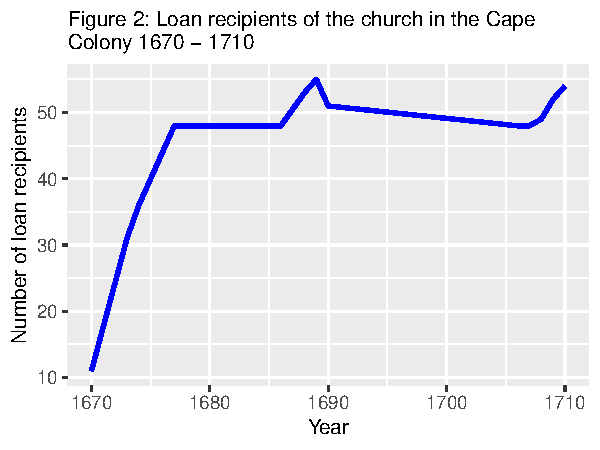
\includegraphics{HistoryEssay_files/figure-latex/unnamed-chunk-2-1} \end{center}

For the number of loan recipients, there is less of a steady increase
over time. Figure 2 depicts that the number of individual loan
recipients in this period increased substantially from 1670 until 1678.
It is evident that after 1678, the number of individual loan recipients
stagnated and approximately 48 recipients received loans from the church
for the remainder of the period and the value only marginally fluctuated
around this level.

\hypertarget{methodology}{%
\section{\texorpdfstring{Methodology
\label{Meth}}{Methodology }}\label{methodology}}

The main research question was to investigate whether there was an
impact of the type of loan recipient on the loan amount granted by the
church. We test the hypothesis that women and manumitted slaves were
likely given smaller loans than others, and Huguenots given greater
loans as they were deemed as beneficial to be a part of Cape Colony
society, which is why the VOC provided inducements to this group of
settlers. To address the aforementioned persistence in the data set,
only the initial observation for each unique loan recipient was included
in the analysis of this paper. This resulted in 144 observations. By
dropping any second observations for a loan recipient, we attempt to
control for the potential multi-collinearity within the data set.
Moreover, we created a dummy for each year included in the data set.
This was necessary because of the general upward trend in the total
amount of loans granted by the church over the time period, as seen in
Figure 1.

To understand the effect of the type of loan recipient on the loan
amount granted by the church, it was necessary to create dummy variables
for the type of loan recipient. The first type identified in the data
set were those with surnames that indicated slave origin, which amounted
to 4 individuals. For example, those with surnames such as `van Guinea'
or `van Bengalen' indicated that these individuals originated from
countries from which slaves were obtained from. It is assumed that these
individuals with slave-origin surnames were manumitted in the Cape
Colony. The second type identified was women. It was rare to find women
in the data set as only 7 women were recorded in the data set, and often
only appeared once. The third type identified was the Huguenots. Using a
list of Huguenot family surnames (Fourie \& von Vintel, 2009), these
loan recipients were categorised and amounted to 12 individuals. The
reference group for all individuals that did not fall into one of these
three aforementioned categories were listed as Other and constituted 128
individuals. It was clear from a preliminary review of the data that
slaves and woman received significantly less loans than Huguenots or
those in the Other category type, in terms of quantity. However, to
investigate whether these types had an effect on the amount of the loan
given by the church was determined using an ordinary least squared
regression, as follows: \[
LoanAmount = x_0 + Huguenot \beta_1 + SlaveOrigin \beta_2 + Woman \beta_3 + YearDummy \beta_i + \varepsilon
\] where the dummy for year is a vector including all the years that
contain initial observations for individual loan recipients, as a
coefficient to beta which is indexed by \(i=4, 5, 6...\).

According to the equation above, a regression was run on all dummies for
both types and years to determine whether there is an effect on loan
amount. Subsequently, two further regressions were run to test the
robustness of the results. A second regression was run in which the type
dummies were dropped and a final third regression was run to include
both the year and type dummies in addition to some interaction terms.

\hypertarget{results-and-discussion}{%
\section{\texorpdfstring{Results and discussion
\label{Discussion}}{Results and discussion }}\label{results-and-discussion}}

In the first regression, the results were that only the coefficients on
the dummies for years 1673, 1675 and 1710 were statistically
significant. The R-squared was found to be 0.218 and the intercept,
which represents the reference group for the `other' type in 1706, had a
coefficient of 659.011. Therefore, if an `other' loan recipient received
a loan in 1673, it is estimated to be 264.063 guldens less than the
reference group. It is interesting to note that the coefficient on the
year 1675 is smaller than for 1673, which is counter-intuitive to the
general upward trend demonstrated in Figure 1. Lastly, there was a
significant and large, positive effect of receiving a loan from the
church in 1710.

In the second regression, only the year dummies were included. This
caused the R-squared to decrease to 0.205, which may indicate that by
dropping the type dummies, some explanatory information has been lost.
However, it is likely because R-squared may be increased simply by
adding parameters, albeit even if they are insignificant parameters. The
years 1708 and 1710 were found to be significant and positive. Lastly,
in the third regression, the inclusion of some interaction terms did
increase the R-squared, but it is likely driven by the aforementioned
parameter effect. The coefficient on the type dummies were still found
to be insignificant for the effect of loan recipient type on loan amount
when interacted with year dummies.

It is an unexpected result to find that woman and those of slave origin
were found to have no negative effect on the loan amount received from
the church, albeit that it there were only few individual loan
recipients who were categorised into these two groups from the data set.
The fact that woman only appeared to receive loans on behalf of their
late husbands can explain why they did not receive lower loan amounts
than men. This demonstrates that the church simply granted loans of the
same value to the late husbands' family in his absence.

The null effect of slaves on loan amounts is likely reflective of the
new regulations enacted in 1685 in the Cape Colony by the
Governor-General van Drakenstein, who was a colonial administrator for
the VOC. It was decided that those slaves who had been manumitted had
become burdensome in terms of the church's funds. Thereby, these new
regulations specified that only those slaves deemed to be
`well-conducted' may be allowed to become manumitted (Wirgman, 1895:33).
Therefore, those who were previously slaves in the Cape Colony after
1685 were deemed to be respectable and were likely treated as such in
society, and by extension the church did not unduly discriminate against
them in the amount of loans granted to these individuals.

With regards to the Huguenot type, as aforementioned in section 2, the
Huguenots were initially seen as an asset to the Cape Colony. However,
the Commander of the VOC in the 1680s did not regard the Huguenot's
assisted emigration favourably, because his policy approach was to align
the Cape Colony more closely with the Netherlands (Wirgman, 1895:36).
Perhaps there was initial favoritism towards the Huguenots, that later
soured into discrimination following the change in leadership's
sentiment, thereby negating any advantage they may have gained from the
church in terms of loan amounts.

\hypertarget{limitations}{%
\section{\texorpdfstring{Limitations
\label{Limitations}}{Limitations }}\label{limitations}}

One limitation of this paper is that the sample of different loan
recipients is relatively small, as only 144 unique loan recipient
observations were recorded. In an attempt to remove multi-collinearity
between years, the sample was made smaller which reduced potential
variation in the data set. Due to the lack of information about each
loan recipient included in the church loan books, a further limitation
of this paper's analysis is omitted variable bias. The reference dummy
category for those who fell into the `other' loan recipient type likely
included further variation that was otherwise difficult to further
specify. Despite searching each loan recipients' full name on genealogy
websites, there was very little information about what may have
distinguished this category. Therefore, if there is some further
categorisation within the `other' type that may have had an effect on
the loan amount, the results may be biased.

As aforementioned, there are many years missing in the church loan
books. It can be assumed that year on year, an omission of a singular
year may not bias our results on average. However, a concern arises
regarding the longer time periods for which there is no record of loans.
For example, in this particular data set there are two large gaps: from
1678 to 1686 and from 1690 to 1706. The reason for concern in the case
of the methodology applied in this research is that the observations
included were only the first loan recorded to a unique loan recipient.
Accordingly, it is likely that after a long period of missing years, the
following available year will be upward biased in terms of its impact on
the loan amount. This can be seen in the fact that 1706 was the
reference group for the year dummy, indicating it was the group with the
highest frequency of observations.

Lastly, there is a selection issue in this paper, as only those who
received loans from the church were included in the sample. Those who
were denied loans from the church were not reflected. This may partly
explain why we see no effect of the type of loan recipients in the
analysis because there may have been a selection by the church to only
provide loans to those they deemed to be needy or respectable within
society. However, the data on those who were not granted loans from the
church does not exist so this analysis made use of the available data to
achieve results for those who were granted loans in the first instance.

\newpage

\hypertarget{conclusion}{%
\section{\texorpdfstring{Conclusion
\label{Conclusion}}{Conclusion }}\label{conclusion}}

To conclude, this paper finds that there was no impact of the type of
loan recipient on the loan amount granted by the church in the Cape
Colony during the period 1670 to 1710. The results found contradict our
preliminary hypothesis that there would be smaller loans granted to
woman and manumitted slaves and larger loans granted to Huguenots on
average, compared to those not included in these groups. It is suggested
that women who received loans from the church were not granted smaller
loans because they received the same loan amounts on behalf of their
late husbands the in years following their husbands death. On the other
hand, the reason for manumitted slaves receiving similar loan amounts
compared to other loan recipients is likely related to the requirements
for manumitted slaves to be deemed as `respectable' in society before
they were freed. Therefore, any discrimination by the church and the VOC
may be mitigated against this requirement. Lastly, the Huguenots were
likely not granted larger loans because they were given favourable
inducements by the VOC to migrate before arrival in the Cape. As a
result, the Commander of the VOC at the time may not have wanted to
advantage this group further because they were not Dutch and he wished
the Colony to be further aligned with the Netherlands. It is suggested
that for further research, the likelihood of receiving more loans
year-on-year for subsequent periods in the data set (for years without
significant gaps) be investigated. Alternatively, potential
discrimination by the church may not have manifested in the amount of
the loans given, but rather in higher interest levied on freed slaves
than for free men.

\newpage

\hypertarget{references}{%
\section*{References}\label{references}}
\addcontentsline{toc}{section}{References}

Fourie, J. \& Von Fintel, D. 2009. The dynamics of inequality in a newly
settled, pre-industrial society: The case of the Cape Colony.
Stellenbosch Economic Working Papers 17. Stellenbosch University.

Fourie, J., Jansen, A. \& Siebrits, K. 2012. Public finances under
private company rule: The Dutch Cape Colony (1652-1795). New Contree,
68:51-71.

Fourie, J. \& Luiten van Zanden, J. 2012. GDP in the Dutch Cape Colony:
The national accounts of a slave-based society. Working Paper No.~4,
Stellenbosch University, Department of Economics.

Fourie, J. 2013. The remarkable wealth of the Dutch Cape Colony:
Measurements from eighteenth-century probate inventories. \emph{The
Economic History Review}, 66(2):419--448.

Guelke, L. 1988. The Anatomy of a Colonial Settler Population: Cape
Colony 1657-1750. \_The International Journal of African Historical
Studies, 21(3):453-473.

Horner, D. \& Wilson, F. 2008. A Tapestry of People: The Growth of
Population in the Province of the Western Cape. A Southern Africa Labour
and Development Research Unit Working Paper No 21. Cape Town: SALDRU,
University of Cape Town.

Wirgman, A. T. 1895. The History of the Church in South Africa
{[}Online{]}.
\url{https://repository.up.ac.za/bitstream/handle/2263/12783/002_p13-49.pdf?sequence=6\&isAllowed=y}
{[}2022, May 19{]}.

\hypertarget{appendix}{%
\section*{Appendix}\label{appendix}}
\addcontentsline{toc}{section}{Appendix}

\hypertarget{regression-1}{%
\section*{Regression 1}\label{regression-1}}
\addcontentsline{toc}{section}{Regression 1}

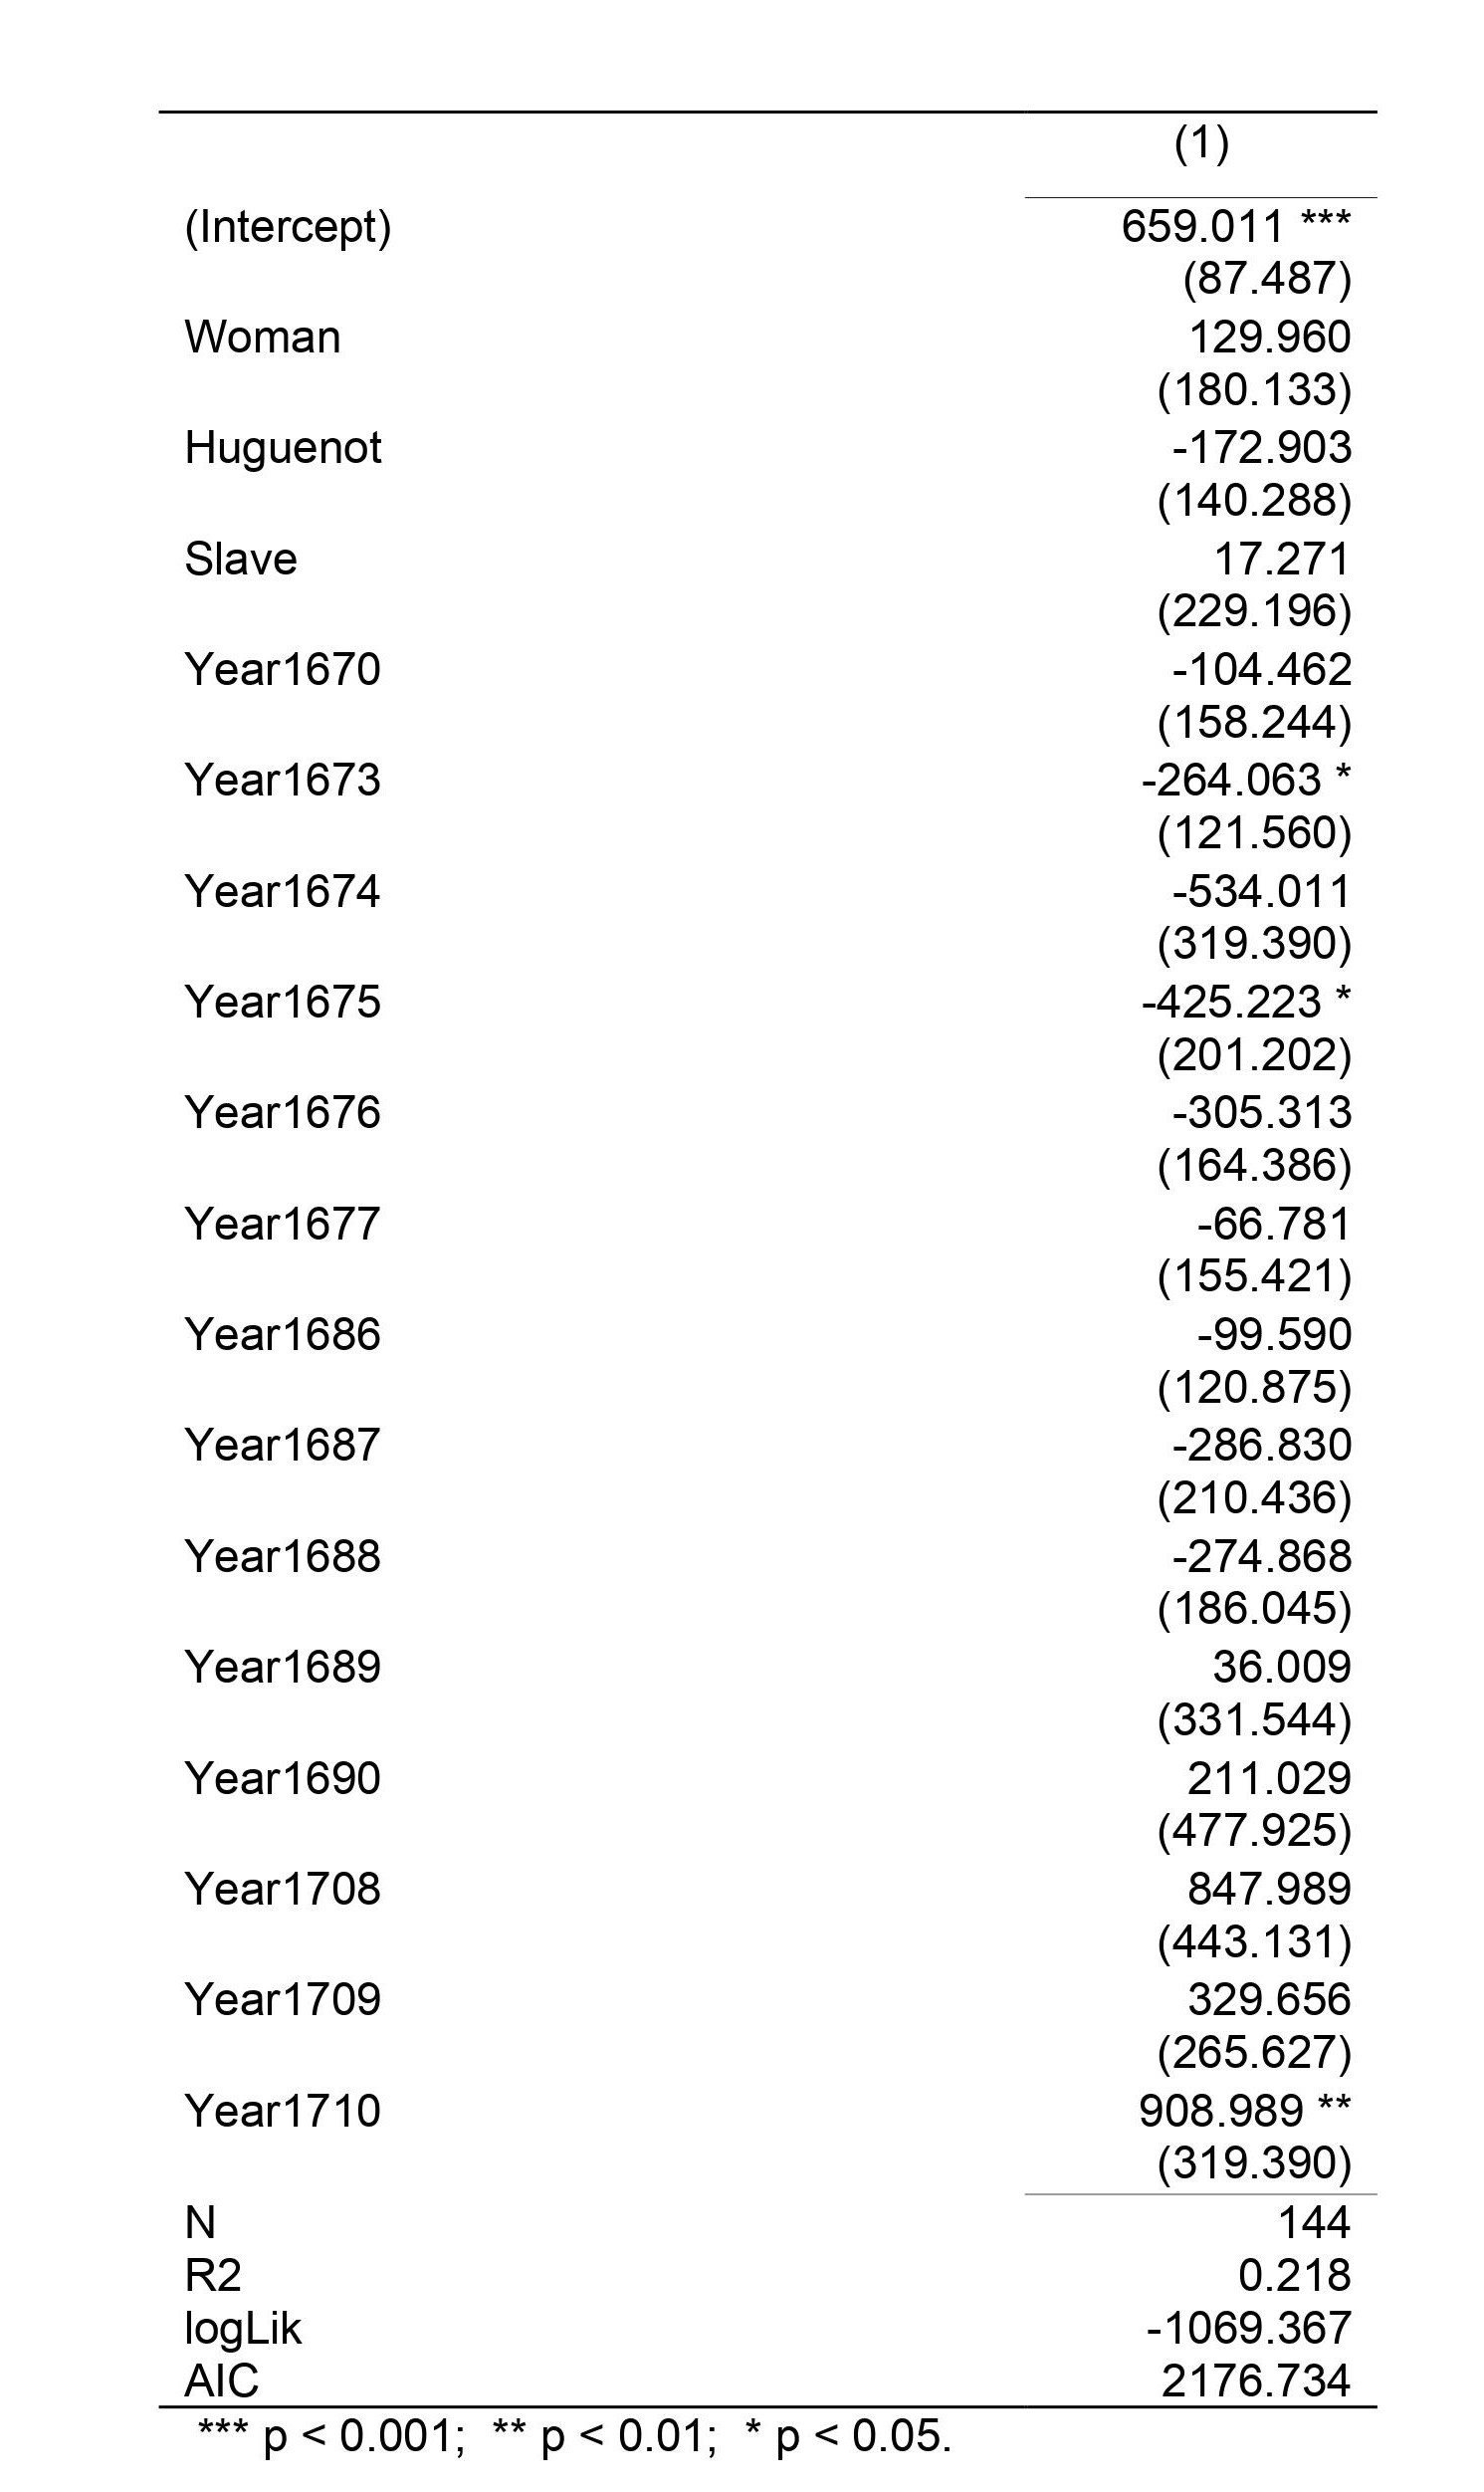
\includegraphics{/Users/Harriet/Documents/Economic History/ESSAY/Texevier_History_Essay/HistoryEssay/data/Reg1.jpg}
\newpage

\hypertarget{regression-2}{%
\section*{Regression 2}\label{regression-2}}
\addcontentsline{toc}{section}{Regression 2}

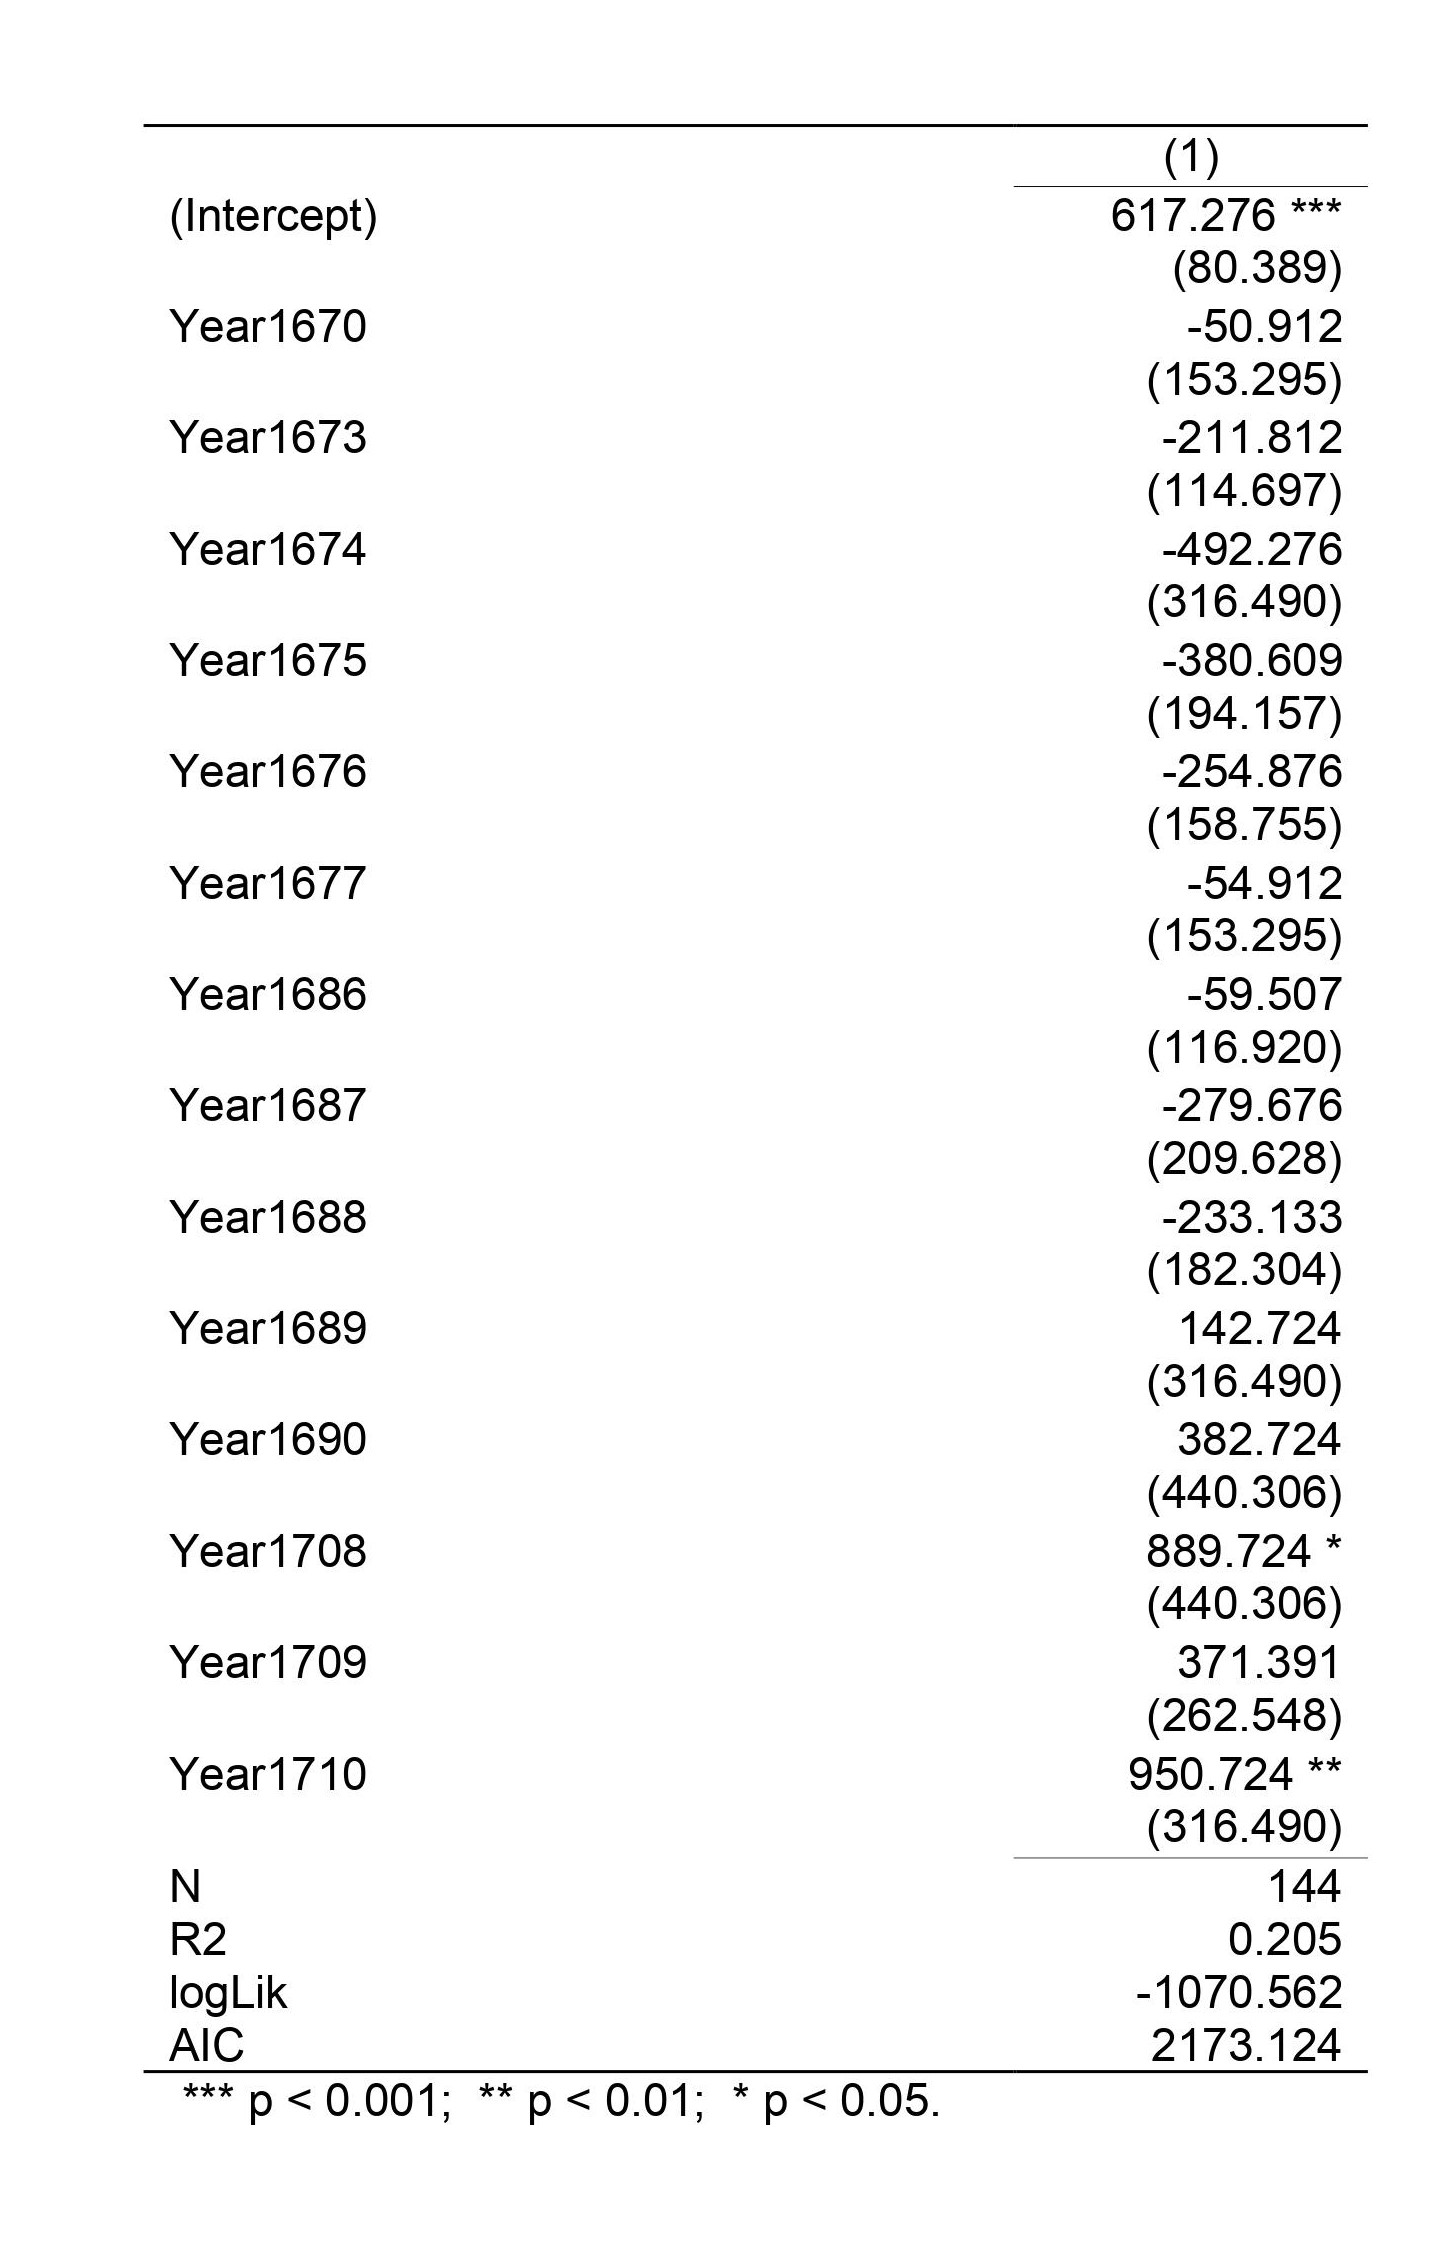
\includegraphics{/Users/Harriet/Documents/Economic History/ESSAY/Texevier_History_Essay/HistoryEssay/data/REg2.jpg}
\newpage
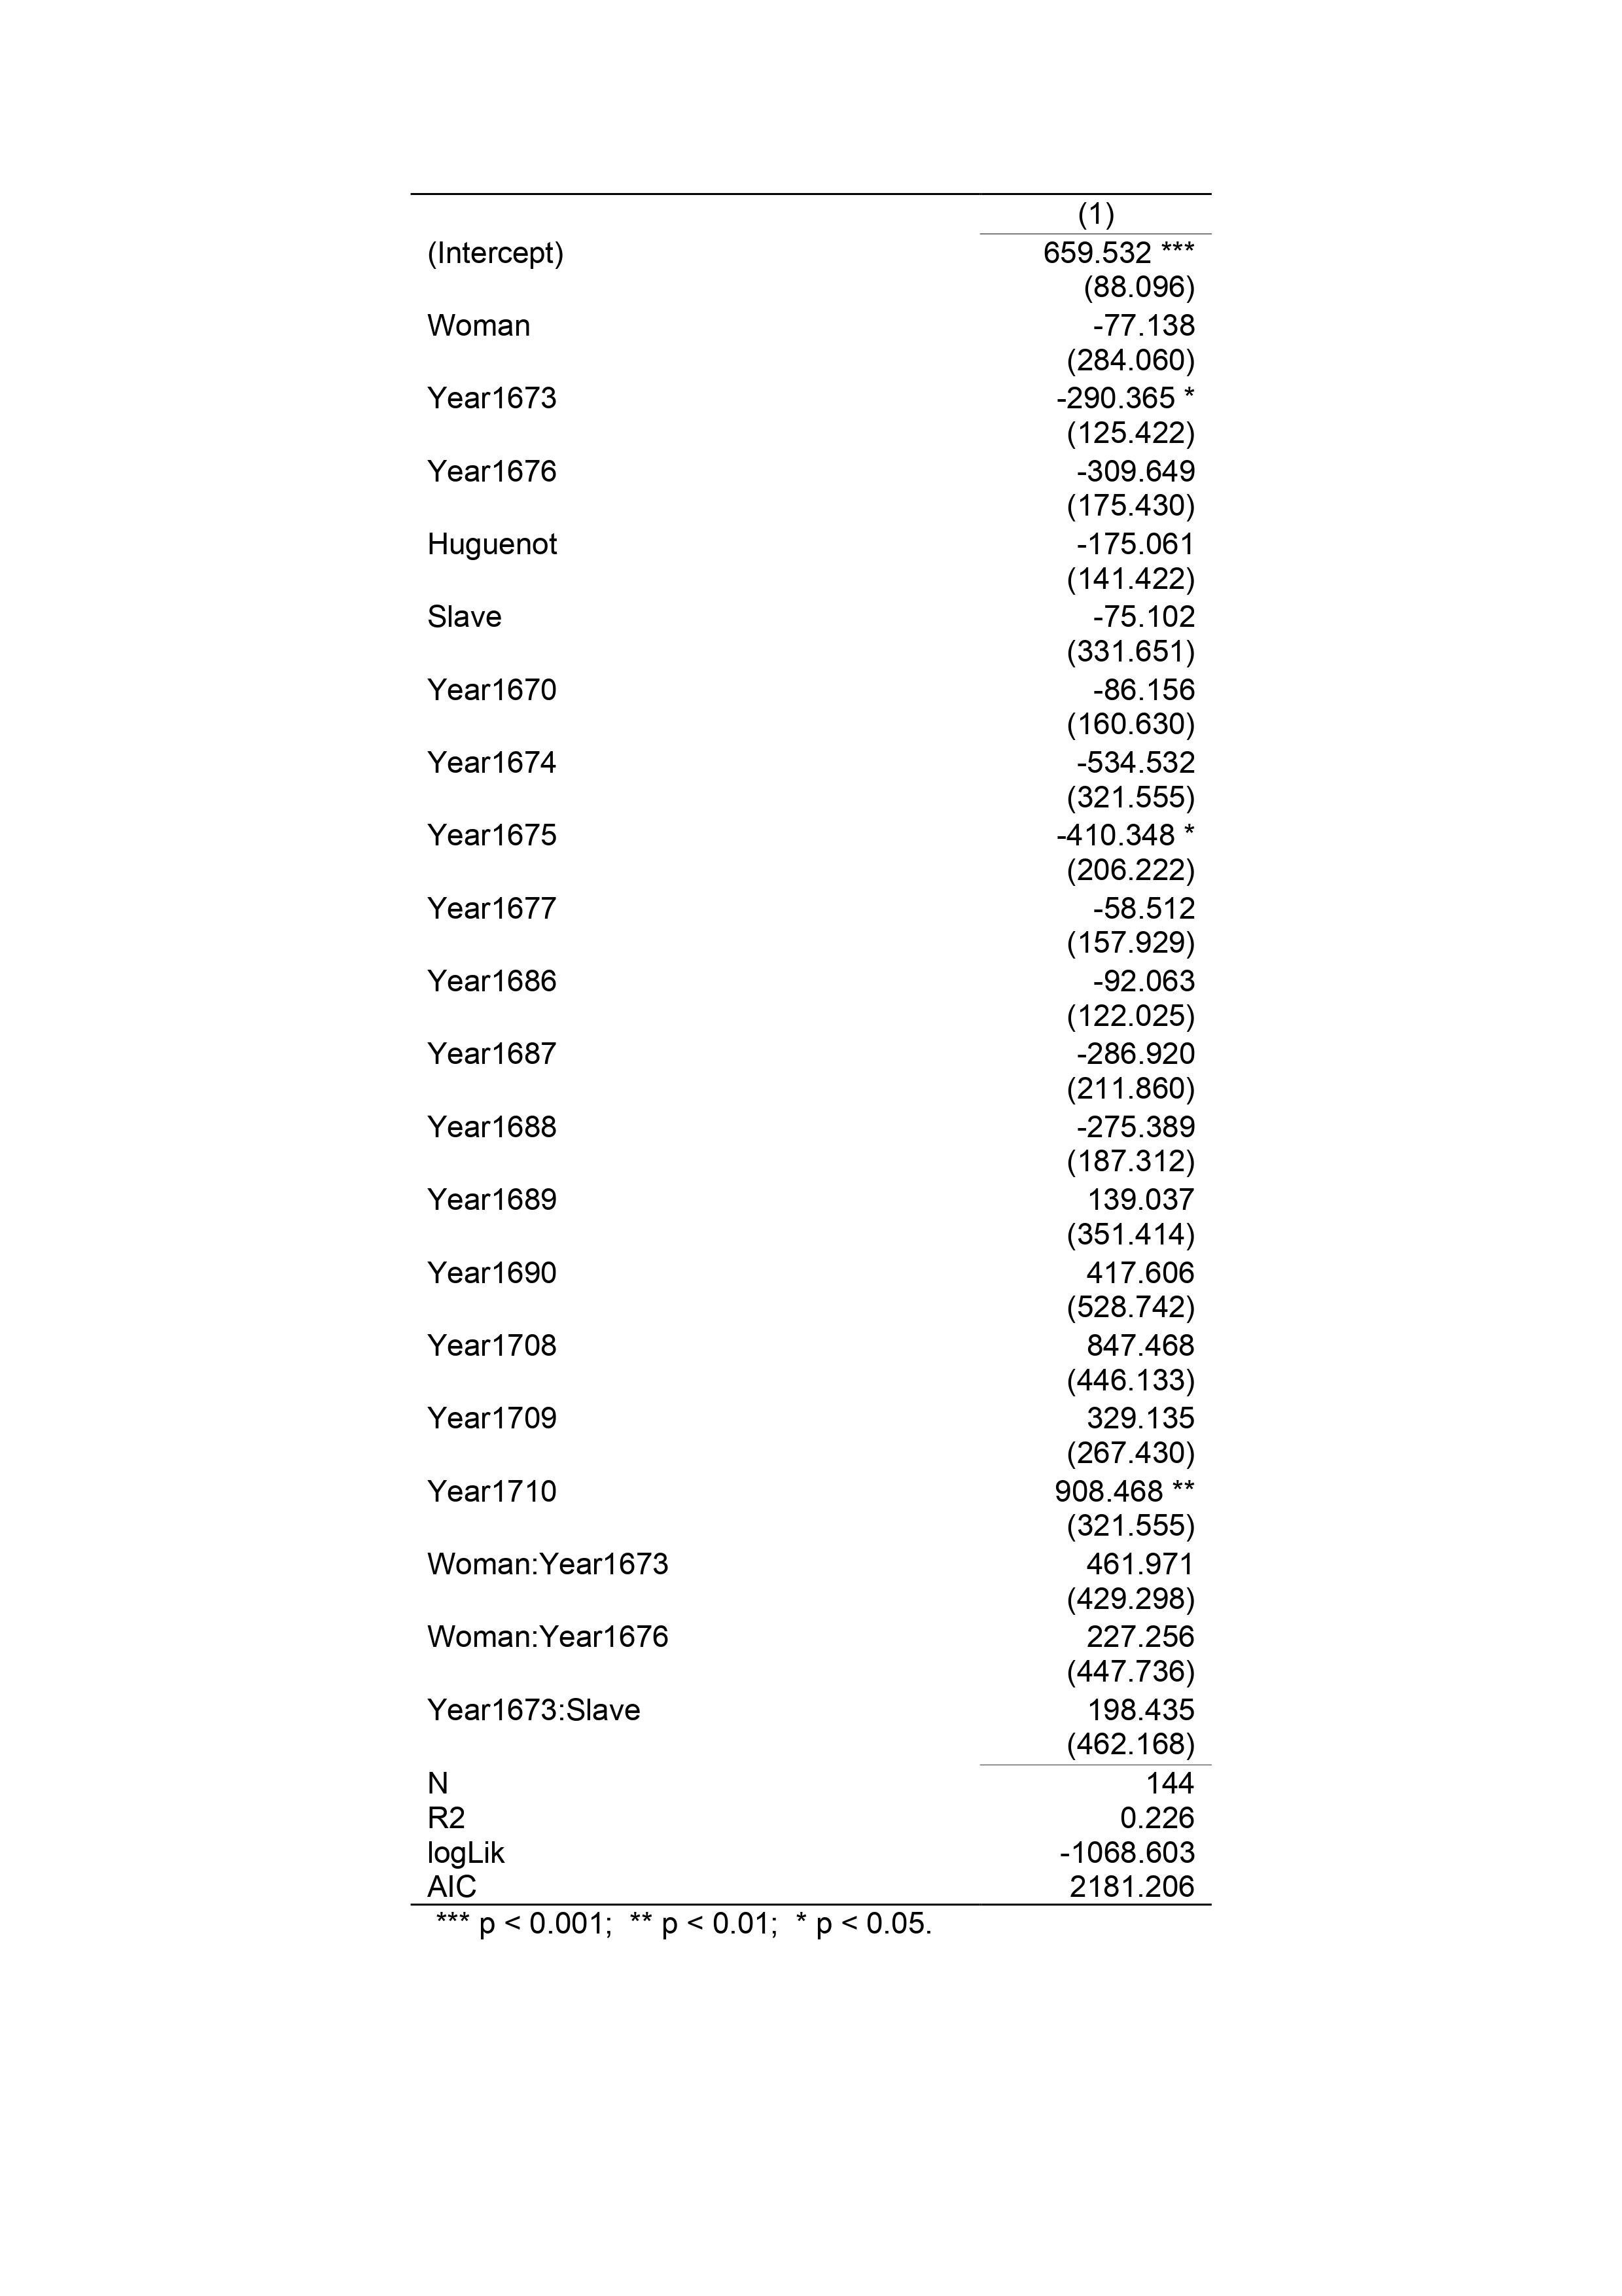
\includegraphics{/Users/Harriet/Documents/Economic History/ESSAY/Texevier_History_Essay/HistoryEssay/data/Reg3.jpg}

\bibliography{Tex/ref}





\end{document}
